\documentclass{beamer}

\year=2023
\month=7
\day=11

\usetheme{simple}
\setbeamertemplate{items}[circle]
\setbeamertemplate{section in toc}[sections numbered]
\setbeamerfont{footnote}{size=\scriptsize}
\def\bibfont{\tiny}
\usepackage{lmodern}
\usepackage[scale=2]{ccicons}

\title{Detección de noticias falsas usando Procesado de Lenguaje Natural}
% \subtitle{Trabajo de Fin de Grado}
\date{\today}
\author{Miguel Ricardo Claramunt Argote}
\institute{Escola Tècnica Superior d'Enginyeria -- Universitat de València}

\begin{document}

\setwatermark[hoffset=0.02\textwidth,voffset=0.02\textwidth]{\includesvg[width=0.7\textwidth]{img/ETSE_2_linies.svg}}
% Title page frame
\begin{frame}
    \titlepage 
\end{frame}

\setwatermark[voffset=0.03\textwidth]{\includesvg[height=0.06\textwidth]{img/ETSE_icono.svg}}

% Outline frame
\begin{frame}{Esquema de la presentación}
    \tableofcontents
\end{frame}

\section{Introducción}
\begin{frame}{1.1. Introducción}

Las \textit{fake news} son piezas de texto con estilo pseudoperiodístico que tienen como objetivo desinformar a los lectores.

% \vspace{2ex}

% Estas `noticias' toman relevancia mundial en las elecciones presidenciales de E.E.U.U. en 2016, superando en \textit{engagement} a los medios tradicionales.

\vspace{2ex}

Motivos principales que incentivan la difusión de \textit{fake news}:
\begin{itemize}
    \item \underline{\smash{Económico:}} publicidad en la página web.
    % y el tráfico que generan estos sitios, pueden generar hasta 30.000 \$ mensuales.\footnote{\citep{Sydell2016}}
    \item \underline{\smash{Ideológico:}} apoyo de una agenda política.\footnote{\citep{AlcottGentzkow2017, Sydell2016}}
    % las \textit{fake news} consiguen enturbiar la opinión pública para apoyar una agenda política determinada.
\end{itemize}

\end{frame}

\begin{frame}{1.2. Motivación}

\textit{Fact checking}:
\begin{itemize}
    \item Exhaustivo, laborioso.
    \item Mayoritariamente manual.
    \item Grandes beneficios si se automatiza: \textit{LLMs}.
\end{itemize}

% Las redes sociales han transformado todo el proceso: formato, difusión, `viralidad', \textit{bots}, etc.

% \end{frame}

% \begin{frame}{Motivación}

% Las \textit{fake news}: 
% manipulan la percepción de la realidad, generando desconfianza y conflicto social.\footnote{\citep{CITSa}}

% % \vspace{2ex}

% El \textit{fact checking} es un proceso muy exhaustivo, laborioso y prácticamente manual, por lo se beneficiaría de la automatización.

\vspace{1ex}

% Los \textit{Large Language Models} (LLMs) permiten desarrollar aplicaciones para automatizar partes de este proceso.

% las siguientes aplicaciones: clasificador de noticias verdaderas/falsas, \textit{Information Retrieval}, resumen automático.

\vspace{2ex}

Otros beneficios: reducción de prejuicios en colectivos minorizados, mejora de la imagen del periodismo/periodista, etc.

\end{frame}

\begin{frame}{1.3. Objetivos}

Objetivo principal:
\begin{itemize}
    \item Desarrollar una solución que permita detectar noticias falsas.
    \begin{itemize}
        \item Clasificación a partir de características estilísticas.
        \item Estudio comparativo: cantidad/calidad de información, arquitectura/tamaño de los modelos. 
    \end{itemize}
\end{itemize}

\vspace{2ex}

Objetivos transversales:
\begin{itemize}
    \item Definición del término de \textit{fake news} y discutir las implicaciones en nuestro trabajo.
    \item Conocer en profundidad cómo funcionan los modelos y los sesgos implícitos.
    \item Aplicación de técnicas de \textit{Explanable AI} (XAI) para intentar entender el `razonamiento' de los modelos.
    % \item Conocer los sesgos de los modelos y cómo afectan la arquitectura y el aprendizaje en estos.
\end{itemize}

\end{frame}

\section{Definiciones}
\begin{frame}{2. Definiciones y área de estudio}

% Diferentes formulaciones del concepto aplicadas a noticias \citep{AlcottGentzkow2017,Lazer2018}.

% \vspace{2ex}

% \citet{Mourao2019} encuentran que la mayoría de información que se difunde no sigue la estructura de una noticia, por lo que hace falta reformular el concepto.

% \vspace{2ex}

% A partir del trabajo de , utilizamos la siguiente definición:

% \vspace{2ex}

\begin{quotation}
    \underline{Disinformation (Desinformación).} Contenido proposicional de signos que tergiversa el estado del mundo con la intención de engañar. --- \citep{Khan2021}   
\end{quotation}

\vspace{2ex}

Problema complejo, límite del area de aplicación a noticias:
\begin{itemize}
    \item \underline{\smash{Recopilables:}} gran disponibilidad de BBDD.
    \item \underline{\smash{Categorizables:}} aprendizaje supervisado.
\end{itemize}

% Ya que el problema es complejo, limitamos el área de aplicación a noticia, que son fácilmente recopilables y categorizables, ayudando al entrenamiento supervisado de los modelos.

\end{frame}

\section{Estado del arte}
\begin{frame}{3. Antecedentes y tecnologías}

% El problema no se conceptualizó hasta la publicación de los trabajos de \citet{Cohen2011, Flew2012}, motivado por los avances en el procesado del lenguaje natural, bases de datos e \textit{information retrieval} de la época.

Se han desarrollado dos enfoques para abordar este problema:
\begin{itemize}
    \item \underline{\smash{Basado en patrones:}}  estilo o sintaxis, métricas de RRSS, minería de datos enfocada a emociones.
    \item \underline{\smash{Basado en evidencias.}} similaridad semántica entre \textit{claim} y evidencia.
\end{itemize} 

\vspace{2ex}

Trabajos relevantes: 
\begin{itemize}
    \item DeClarE \citep{Popat2018}
    \item HAN \citep{Ma2019}
    \item GET \citep{Xu2022}
\end{itemize}

\end{frame}

% \begin{frame}{Tecnologías}

% \textbf{DeClarE \citep{Popat2018}.} Basado en evidencias, utiliza redes neuronales convolucionales (CNN) para extraer características locales de las evidencias y contraevidencias; mientras que usa redes recurrentes (RNN) para capturar dependencias entre diferentes evidencias.


% \textbf{HAN \citep{Ma2019}.} Basado en patrones, extrae las \textit{features} mediante una \textit{Hierarchical Attention Network} (HAN) que extrae relaciones a nivel de palabra y a nivel de oración.

% \vspace{4ex}

% \textbf{GET \citep{Xu2022}.} Unifica los dos enfoques y propone una solución utilizando grafos, que permiten capturar dependencias semánticas a larga distancia.

% \end{frame}

\section{Análisis del problema}
\section{Estudio preliminar}

En un principio queríamos analizar el discurso de odio y las \emph{fake news} que se difunden por redes sociales, motivado por los trabajos de \citet{Gomez2019,Toraman2022}.

Algunos de los \textit{datasets} considerados fueron los siguientes:
\begin{itemize}
    \item \underline{VoterFraud2020 \citep{Abilov2021}:} \textit{Dataset} multimodal de \emph{tweets} y \emph{retweets} en inglés que contienen palabras clave y \emph{hashtags} relacionados con alegaciones y reclamaciones sobre fraude electoral en las elecciones presidenciales de Estados Unidos en 2020.
    \item \underline{Hate Speech Corpus:} \textit{Dataset} en inglés obtenido a partir del trabajo realizado por \citet{Szpakowski2017}. Extraen artículos de medios catalogados por publicar contenido de discurso de odio en Internet. Estos artículos tratan anti-semitismo, misoginia, anti-inmigración/xenofobia, homofobia o discurso de odio en general.
    \item \underline{MMHS150K \citep{Gomez2019}:} \textit{Dataset} multimodal en inglés que incluye \emph{tweets} e imágenes relacionadas con discurso de odio.
    \item \underline{Hate + COVID + Temporers \citep{Rodriguez2022}:} \textit{Dataset} de \textit{tweets} en castellano y catalán relacionados con COVID-19 y temporeros en Cataluña, los cuales la mayoría de ellos suelen ser migrantes o pertenecen a poblaciones minorizadas. Los \textit{tweets} se recogieron en el periodo de enero a octubre del 2020, obteniendo un total de 1.062 \textit{tweets}.
\end{itemize}

Debido a que las pruebas de LLMs con estos \textit{datasets} no obtenían resultados satisfactorios, decidimos redirigir la investigación hacia detección de noticias falsas, las cuales tienen estrecha correlación con el discurso de odio. 

Una de las razones por las que creemos que los LLMs no funcionaban con estos \textit{datasets} era por la poca cantidad de texto que contenían en los casos de \citet{Abilov2021,Gomez2019,Rodriguez2022}. Esto se justifica con el hecho de que los datos obtenidos son procedentes de Twitter y en el momento de recolección de los datos existía un límite de 280 caracteres por \emph{tweet}. Al no tener suficiente información de texto por \textit{tweet} y por consecuencia no tener suficiente contexto, suponemos que los LLMs no eran capaces de detectar las características necesarias para realizar la clasificación.

Además, los \textit{datasets} de \citet{Abilov2021,Szpakowski2017} no tenían casos negativos (es decir, muestras que no estuvieran categorizadas como discurso de odio). Esto suponía realizar una creación de un \textit{dataset} de casos negativos, por lo que decidimos finalmente descartar estos \textit{datasets}.


\section{Datasets}

\subsection{Descripción del conjunto de datos}

\subsubsection{Politifact y Snopes}

Snopes \citep{Popat2017} y PolitiFact \citep{Vlachos2014} son dos \textit{datasets} creados a partir de las agencias de \textit{fact-checking} homónimas.

Ambos \textit{datasets} son obtenidos gracias a \citet{Xu2022}, que utilizan ambas páginas para obtener las \textit{claims} y etiquetas para cada noticia (en el caso de Snopes son \textit{True}/\textit{False}). A partir de cada \textit{claim}, obtienen las evidencias y demás información mediante motores de búsqueda. Para el caso de PolitiFact la única diferencia que existe es que se fusionan las clases positivas (\textit{true}, \textit{mostly true} y \textit{half true}) en la categoría \textit{true}, mientras que las negativas (\textit{false}, \textit{mostly false} y \textit{pants on fire}) como \textit{false}. Un último dato relevante sobre este dataset es que está normalizado, por lo que los modelos entrenados con este dataset tendrán solo acceso a la información contextual o estilística de las noticias.

En la figura \hyperref[tab:sp-dataset]{4.1} se pueden encontrar diversas estadísticas sobre el dataset: 
\begin{table}[H]
\centering
\begin{tabular}{ccr}
\hline
\textbf{Dataset} & \textbf{Feature} & \textbf{Conteo} \\ \hline
\multirow{5}{*}{PolitiFact} & True & 1543 \\
 & False & 1565 \\
 & Evidences & 3108 \\
 & Speakers & 137 \\
 & Publishers & 1064 \\ \hline
\multirow{5}{*}{Snopes} & True & 690 \\ \
 & False & 2066 \\
 & Evidences & 2756 \\
 & Speakers & N/A \\
 & Publishers & 1873 \\ \hline
\end{tabular}
\caption{Conteo de muestras según \textit{features}.}
\label{tab:sp-dataset}
\end{table}

\subsubsection{ISOT Fake News Dataset}

Este conjunto de datos contiene artículos periodísticos reales y falsos. Los artículos reales fueron obtenidos de la agencia de noticias Reuters, mientras que los artículos falsos han sido obtenidos de medios poco fiables catalogados por PolitiFact (una agencia de verificación de noticias de EE.UU.) y Wikipedia. 

\begin{table}[htb]
    \centering
    \begin{tabular}{ccrr}
        \hline
        \multirow{2}{*}{\textbf{News}} & \multicolumn{2}{c}{\textbf{Subjects}}                               & \multicolumn{1}{c}{\multirow{2}{*}{\textbf{Total size}}} \\
                                       & \footnotesize{\textbf{Type}} & \multicolumn{1}{c}{\footnotesize{\textbf{Size}}} & \multicolumn{1}{c}{}                               \\ \hline
        \multirow{2}{*}{Real-News} & World-News      & 10145 & \multirow{2}{*}{21417} \\
                                   & Politics-News   & 11272 &                        \\ \hline
        \multirow{6}{*}{Fake-News} & Government-News & 1570  & \multirow{6}{*}{23481} \\
                                   & Middle-East     & 778   &                        \\
                                   & US News         & 783   &                        \\
                                   & Left-News       & 4459  &                        \\
                                   & Politics        & 6841  &                        \\
                                   & News            & 9050  &                        \\ 
        \hline
    \end{tabular}
    \caption{Conteo de muestras según categorías \citep{Ahmed2017}.}
    \label{fig:news-dataset}
\end{table}


Los temas que incluye este \textit{dataset} abarcan diferentes ámbitos, aunque como se puede observar en la figura \ref{fig:news-dataset}, la gran mayoría tratan sobre política y actualidad mundial.

Cada artículo contiene la siguiente información: título del artículo, texto, tipología y fecha de publicación. Las noticias recogidas en este \textit{dataset} están limitadas al periodo entre 2016 y 2017. Posteriormente, estas noticias fueron limpiadas y procesadas, aunque en el caso de las noticias falsas no se corrigieron errores tipográficos, en los cuales se incluyen errores ortográficos o de puntuación. 

Este \textit{dataset} mantiene un equilibrio entre clases, por lo que no es necesario aplicar técnicas de \textit{Data Augmentation}. 

\subsection{Procesamiento del conjunto de datos}

\subsubsection{Politifact y Snopes}

Para trabajar con ambos \textit{datasets} fusionaremos ambos \textit{datasets}, creando una nueva columna \texttt{dataset} que indica si pertenece al \textit{dataset} \texttt{politifact/snopes} (por si es necesario en un futuro análisis). Concatenamos los \textit{strings} para el titular y cuerpo de la noticia.

Debido a que contamos con varias evidencias para el mismo \textit{claim}, generaremos dos \textit{datasets} a partir de este, {P-S}\textsubscript{One} y {P-S}\textsubscript{All}. La diferencia entre ambos es que el primero de ellos contendrá solamente una evidencia, elegida aleatoriamente; el otro contendrá todas las evidencias concatenadas junto al titular, como hemos mencionado anteriormente.

De esta forma, ambos \textit{datasets} {P-S}\textsubscript{One} y {P-S}\textsubscript{All} tendrán el mismo número de muestras, 789, aunque con diferente información, teniendo el \textit{dataset} {P-S}\textsubscript{All} más información contextual sobre el hecho sucedido.

De esta forma, obtenemos estos dos \textit{datasets} con las siguientes características:

\begin{table}[htb]
    \centering
    \begin{tabular}{ccrr}
        \hline
        \textbf{Dataset} & \textbf{Etiqueta} & \multicolumn{1}{c}{\textbf{Conteo}} & \multicolumn{1}{c}{\textbf{Total}} \\\hline
        \multirow{2}{*}{PolitiFact} & True & 186 & \multirow{2}{*}{356} \\
         & False & 170 &  \\ \hline
        \multirow{2}{*}{Snopes} & True & 116 & \multirow{2}{*}{433} \\
         & False & 317 & \\\hline
    \end{tabular}
    \caption{Conteo de muestras según categorías.}
    \label{tab:sp-new}
\end{table}

Podemos observar que existe un pequeño desbalanceo entre clases \textit{True}/\textit{False}, donde la proporción entre noticias falsas y verdaderas es de 3:2 respectivamente. Debido a que este desbalanceo no es tan pronunciado, consideramos que no es necesario aplicar alguna técnica de balanceo entre clases.

Por último, con respecto al \textit{dataset} {P-S}\textsubscript{All}, consideramos pertinente mostrar las siguientes estadísticas sobre el número de evidencias por noticia:

\begin{table}[htb]
    \centering
    \begin{tabular}{cr}
        \hline
        \textbf{Estadístico} & \multicolumn{1}{c}{\textbf{Valor}} \\ \hline
        Media & 7,43 \\
        Desviación estándar & 6,34 \\
        Mínimo & 1 \\
        \text{Q}\textsubscript{1} & 2 \\
        \text{Q}\textsubscript{2} & 5 \\
        \text{Q}\textsubscript{3} & 11 \\
        Máximo & 27 \\\hline
    \end{tabular}
    \caption{Estadísticas con respecto al número de evidencias por noticia.}
    \label{tab:sp-stats}
\end{table}

Como podemos observar, al menos el 75\% de noticias tienen 2 evidencias o más, por lo que aunque los \textit{datasets} \textit{datasets} {P-S}\textsubscript{One} y {P-S}\textsubscript{All} parten del mismo conjunto de datos original, {P-S}\textsubscript{All} tiene considerablemente más información contenida por noticia que su contraparte {P-S}\textsubscript{One}.


\subsubsection{ISOT Fake News Dataset}

En este \textit{dataset} podemos encontrar para las noticias reales que todas comienzan por la ubicación del suceso y la agencia de noticias, de la siguiente forma:

\begin{center}
\begin{BVerbatim*}
`BARCELONA/GIRONA, Spain (Reuters) - '
\end{BVerbatim*}
\end{center}


También es posible encontrar aclaraciones a principio de esta información, como puede ser:

\begin{center}
\begin{BVerbatim*}
`(This Oct. 9 story has been refiled to add a 
dropped word in the headline) By Sonya Dowsett'
\end{BVerbatim*}
\end{center}

Es por ello que hemos borrado estos fragmentos de texto para evitar que el modelo pueda aprender a utilizar estas estructuras y diferenciar entre noticias verdaderas y falsas, ya que en el caso de las falsas esto no sucede.

Como el \textit{dataset} está dividido en dos archivos, cada uno conteniendo las noticias de una label concreta (\textit{True}/\textit{False}), añadimos una columna adicional para codificar la categoría a la que pertenecen y concatenamos ambos \textit{datasets} para obtener el \textit{dataset} final con todas las noticias.

Posteriormente, concatenamos los \emph{strings} para el titular y el cuerpo de la noticia.

\subsubsection{Normalización y limpieza}

Después de haber obtenido los \textit{datasets} procesados con los que vamos a entrenar los modelos, aplicamos un paso adicional de normalización y limpieza de texto para los modelos \textit{Bag of Words} y TF-IDF.

Para ello, aplicamos los siguientes pasos:
\begin{enumerate}
    \item Sustituimos diferentes acrónimos de estados, organizaciones, siglas y palabras malsonantes censuradas por sus equivalentes.
    \item Convertimos el texto a minúsculas
    \item Expandimos contracciones
    \item Eliminamos enlaces web, \emph{tags} HTML, caracteres mal codificados, símbolos de puntuación y otros caracteres indeseados.
    \item Eliminamos \emph{stop words}
    \item Tokenizamos cada palabra
    \item Lematizamos cada token
\end{enumerate}

\subsubsection{Creación de conjuntos de entrenamiento, validación y test}

Para el entrenamiento de los modelos \textit{Bag of Words} y TF-IDF, hacemos uso de la librería \texttt{scikit-learn} \citep{scikit} y hacemos dos conjuntos: entrenamiento y test, debido a que no es necesario un conjunto de validación en esta implementación.

Estos dos conjuntos se dividen en un ratio 8:2 para entrenamiento y test respectivamente. De esta manera, la misma proporción de muestras se dedican al entrenamiento para estos modelos como para los \textit{transformers}.

En el caso del entrenamiento de los modelos basados en \textit{transformers}, aprovechamos la clase \texttt{Dataset} de la librería \texttt{datasets} \citep{datasets} y creamos tres conjuntos: entrenamiento, validación y test. Como hemos adelantado, la división se hace de forma 8:1:1 respectivamente; evitando que ninguno de los modelos tengan acceso a un mayor número de muestras durante su entrenamiento.

\section{Modelos y clasificadores utilizados}

\subsection{Bag of Words}

Es una técnica de representación de documentos la cual se basa en contabilizar el número de veces que aparece cierta palabra en el documento. De esta forma, dos documentos serán similares si contienen las mismas palabras \citep{Vajjala2020}. Este modelo es denominado de esta manera ya que solamente incluye información sobre el conteo de cada palabra, ignorando cualquier información (gramatical, contextual, etc.) a excepción de las palabras en si \citep{Eisenstein2019}.

\subsection{TF-IDF}

TF-IDF modela la información de forma similar al modelo \textit{Bag of Words}, ya que no almacena ningún tipo de información gramatical o contextual. Lo novedoso de este modelo es que introduce los conceptos de \textit{term-frequency} y \textit{inverse document frequency}.

Se basa en el siguiente hecho: si una palabra concreta aparece repetidas veces en un documento pero no en el resto, entonces esta palabra debe ser importante o representativa para ese documento. Es por ello que la importancia de una palabra determinada debe incrementarse proporcionalmente a su frecuencia en un documento determinado; también, esta debe disminuir proporcionalmente a su frecuencia en otros documentos del corpus \citep{Vajjala2020}.

Matemáticamente, esta relación es capturada usando la \textit{term-frequency} y \textit{inverse document frequency}, que combinadas generan el \textit{TF-IDF score}.

TF \textit{(term-frequency)} mide la frecuencia de una palabra $p$ en un documento $d$.

IDF \textit{(inverse document frequency)} mide la importancia de una palabra $p$ en el corpus, dando más peso a las palabras menos frecuentes (o las más inusuales). Se define como:

\begin{equation}
    \text{IDF}(p, D) = \ln{\frac{D}{\lvert\left\{d\in D: p \in d\right\}\rvert}}
\end{equation}

Siendo $D$ el número total de documentos en el corpus y $\lvert\left\{d\in D: p \in d\right\}\rvert$ el número de documentos donde la palabra $p$ aparece.

Finalmente el \textit{TF-IDF score} se calcula de la siguiente manera:

\begin{equation}
    \text{TF-IDF}(p, d, D) = \text{TF}(p, d) \cdot \text{IDF}(p, D)
\end{equation}

\subsection{Regresión logística}

La regresión logística es un método estadístico que modela la relación entre una variable dependiente y una o más variables independientes. Se utiliza para problemas de clasificación binaria.

Para tareas de clasificación de texto, la regresión logística funciona calculando una suma de las características de entrada (en nuestro caso la representación mediante \textit{Bag of Words} o TF-IDF) y calculando mediante una función logística el resultado. 

El modelo de regresión logística toma los valores de entrada y aprende a predecir la probabilidad de cada clase basándose en las características de entrada. El modelo hace esto aprendiendo un conjunto de pesos para cada característica que se utilizan para calcular una suma ponderada de las características de entrada. Esta suma ponderada se pasa luego a través de la función logística para producir un valor de probabilidad para cada clase.

\subsection{Naïve Bayes}

Naïve Bayes es un algoritmo probabilístico basado en el teorema de Bayes. Establece que la probabilidad de una hipótesis (en este caso, una clase) es proporcional a la probabilidad de la evidencia (en este caso, las características de entrada) dada esa hipótesis.

En la clasificación de texto, Naïve Bayes funciona calculando la probabilidad de cada clase dada las características de entrada. Lo hace asumiendo que las características de entrada son condicionalmente independientes dadas las clases. Esta suposición se llama suposición `ingenua'\ o `naïve', y es lo que le da al algoritmo su nombre.

El algoritmo Naïve Bayes luego calcula la probabilidad de cada clase dada las características de entrada utilizando el teorema de Bayes. Específicamente, calcula la probabilidad previa de cada clase (es decir, la probabilidad de cada clase antes de ver ninguna evidencia), y luego multiplica esto por la verosimilitud de la evidencia dada cada clase (es decir, la probabilidad de ver las características de entrada dadas cada clase). Finalmente, normaliza estas probabilidades para obtener una distribución de probabilidad sobre las clases.

\subsection{SVM y SGD}

Estos métodos supervisados funcionan aprendiendo una función que mapea las características de entrada a las clases de salida. Por esta razón, son similares a la regresión logística.

Las máquinas de vectores de soporte (SVM) son un tipo de clasificador que funcionan encontrando el hiperplano que separa al máximo las características de entrada en diferentes clases. El hiperplano se elige de manera que maximice el margen entre las clases. El margen se define como la distancia entre el hiperplano y los puntos de datos más cercanos de cada clase.

La función de pérdida del perceptrón es un tipo de función de pérdida que se utiliza para entrenar SVM. Funciona minimizando la distancia entre la salida predicha y la salida verdadera. Específicamente, minimiza la suma de las distancias entre cada salida predicha y su correspondiente salida verdadera.

\subsection{Random Forest}

El algoritmo Random Forest funciona construyendo múltiples árboles de decisión y luego combinando sus predicciones.

Cada árbol de decisión se construye seleccionando aleatoriamente un subconjunto de las características de entrada y luego particionando recursivamente los datos en función de estas características. La partición se realiza de tal manera que los subconjuntos resultantes sean lo más puros posible con respecto a las clases de salida.

Una vez que se han construido todos los árboles de decisión, sus predicciones se combinan para obtener una predicción final. Esto se hace típicamente tomando una mayoría de votos sobre todos los árboles de decisión.

\subsection{BERT}

\citet{Devlin2018} discute que las técnicas de aprendizaje hasta el momento limitan las capacidades de los LLMs, concretamente ELMo \citep{Peters2018} y GPT \citep{Radford2018} tienen una forma de aprendizaje unidireccional. Esto puede mermar tareas como \emph{question answering}, las cuales se benefician de disponer de contexto por ambos lados.

BERT está basado en la arquitectura de los Transformers propuesta por \citet{Vaswani2017} y propone una arquitectura bi-direccional en la cual el modelo aprenderá siguiendo estas dos tareas:

Inspirados en la Prueba cloze o \emph{Cloze test} \citep{Taylor1953}, se enmascaran una parte de los \emph{tokens} en el texto para que el modelo prediga cuál va en su lugar; esta tarea la denominan como \emph{Masked LM} (MLM). Esta tarea se distingue de los \emph{denoising auto-encoders} en el hecho de que el objetivo consiste en predecir el \emph{token} enmascarado, en lugar de reconstruir completamente el \emph{input}.

La segunda tarea que desempeña el modelo en su entrenamiento es la denominada \emph{Next Sentence Prediction} (NSP). A partir de un par de frases, el modelo debe clasificar si la segunda frase es continuación de la primera.

\subsection{DistilBERT}

DistilBERT \citep{Sanh2019} se basa en el concepto de \emph{Knowledge Distillation}, donde un modelo compacto `alumno'\ es entrenado para reproducir el comportamiento del modelo `profesor', de mayor tamaño.

Siguiendo una arquitectura del modelo `profesor', el modelo `alumno' tiene una arquitectura similar aunque reducida en el número de capas, el cual se reduce a la mitad. 

Otro truco se aplica en la inicialización de los parámetros del modelo `alumno': aprovechando que la arquitectura de ambos modelos es similar y por lo tanto su dimensionalidad también es similar, aprovechan los pesos del modelo `profesor' para inicializar los pesos del `alumno'.

En resumen, DistilBERT consigue reducir el tamaño del modelo en un 40\% y la complejidad de computación en un 60\%, reteniendo el 97\% de capacidades del modelo original.

\subsection{RoBERTa}

RoBERTa \citep{Liu2019} mejora el rendimiento de BERT mediante mejoras en el proceso de aprendizaje y mejora de hiperparámetros, ya que descubrieron que este estaba infra-entrenado. Es por ello que proponen los siguientes cambios con respecto a la arquitectura y el proceso de entrenamiento:

Primero, descartan el entrenamiento mediante \emph{Next Sentence Prediction}, ya que consideran que su contribución mina el rendimiento global del modelo. Es por ello, que después de diversos experimentos llegan a la conclusión que eliminando esta tarea se consiguen rendimientos iguales o mejores, por lo que se puede prescindir perfectamente de esta tarea.

La siguiente modificación tiene relación con el valor del \emph{learning rate} y el \emph{batch size}. El trabajo de \citet{Ott2018} dejan entrever que aumentar el \emph{batch size} permite una aceleración en el aprendizaje además de una mejora en el rendimiento del modelo, siempre y cuando el valor del \emph{learning rate} se ajuste acordemente. Por otro lado, también se ha descubierto que BERT se puede aprovechar de este tipo de entrenamiento \citep{You2019}. 

Motivado por los trabajos mencionados anteriormente, \citet{Liu2019} aumenta \emph{batch size} de 256 llegando hasta 8.192 muestras por \emph{batch}, obteniendo mejoras en los valores de \emph{perplexity} y rendimiento en tareas finales.

Por último, la última mejora propuesta se enlaza con la tarea de \emph{Masked LM}: se mejora el proceso de enmascarado de los \emph{tokens}: en el caso de BERT este enmascarado es estático, enmascarando solo un tipo determinado de \emph{tokens}. El enmascarador dinámico de RoBERTa enmascara diferentes tipos de \emph{tokens} según cada época en el entrenamiento, haciendo que el modelo sea menos dependiente en los patrones de las frases y por tanto más robusto.

Después de comentar los diferentes aspectos con respecto al proceso de entrenamiento, solamente quedaría mencionar el corpus utilizado. Inspirado por el trabajo de \citet{Yang2019}, decidieron utilizar también un corpus considerablemente grande, sobre unas 10 veces más grande que el utilizado para entrenar BERT. Esto resulta ser idóneo para obtener un buen rendimiento en el modelo sin dar indicios de sobreajuste.

\subsection{DeBERTa}

DeBERTa \citep{He2020} propone una mejora en la arquitectura de BERT \citep{Devlin2018} la cual se basa en el principio de \emph{Disentangled Attention}:

En el caso de BERT, cada palabra en la capa de \emph{inputs} es representada en forma de vector como la suma del valor del \emph{word embedding} y \emph{position embedding}. DeBERTa propone trabajar estos dos valores por separado y calcular los valores de atención mediante \emph{disentangled matrices}, teniendo en cuenta estos valores de posición y contenido.

Esto se justifica en el hallazgo de que la atención para un par de palabras depende tanto del contenido de las palabras como de su posición relativa entre ellas.

Mediante este novedoso mecanismo de atención, DeBERTa consigue mejorar el rendimiento de BERT y RoBERTa, especialmente en tareas que requieren un razonamiento exhaustivo de diferentes partes de la \emph{input}.


\section{Material, recursos utilizados e implementación}

El trabajo realizado en este proyecto se ha desarrollado en Python 3.9 \citep{python}, utilizando Jupyter Notebook \citep{jupyter} como interfaz de programación principal para la implementación. El código ha sido desarrollado y probado a pequeña escala en un ordenador de tipo usuario, mientras que el grueso del entrenamiento, evaluación y testeo de los modelos ha sido ejecutado en un servidor proporcionado por la Universitat de València.

Las librerías utilizadas fueron las siguientes: \texttt{pandas} \citep{pandas}, \texttt{numpy} \citep{numpy}, \texttt{scikit-learn} \citep{scikit}, \texttt{nltk} \citep{nltk}, \texttt{pytorch} \citep{pytorch}, \texttt{transformers} \citep{transformers}, \texttt{datasets} \citep{datasets}, \texttt{shap} \citep{SHAP}.

Por otro lado, las especificaciones del servidor provisto son las siguientes:
\begin{itemize}
    \item 1x Intel\textsuperscript{\textregistered}  Xeon\textsuperscript{\textregistered} CPU E5-2650 v4 @ 2.20GHz
    \item 264 GB RAM DRR4
    \item 1x NVIDIA\textsuperscript{\textregistered}  Tesla\textsuperscript{\textregistered} P100-PCIE-12GB
\end{itemize}

El \emph{script} de entrenamiento de los modelos tardó en ejecutar un total de 2 días y 13 horas de forma ininterrumpida, ya que se ejecutó con el comando \texttt{nohup} \citep{coreutils}. El resto del código implementado ha sido ejecutado de forma \emph{online} con Jupyter Notebook debido a las facilidades que aporta.


% \section{Metodología aplicada}
% % \begin{frame}{Metodología aplicada}

% \textbf{Entrenamiento de modelos estadísticos:} utilizamos la librería \texttt{scikit-learn}\footnote{\citep{scikit}}, entrenamos el vectorizador y el clasificador con el conjunto de entrenamiento. Determinamos una serie de parámetros para los vectorizadores y después de entrenar los modelos y los clasificadores, realizamos las predicciones con el conjunto \textit{test}.

% \vspace{2ex}

% \textbf{Entrenamiento de \textit{transformers}:} utilizamos de la librería \texttt{transformers}\footnote{\citep{transformers}} su \textit{tokenizer} correspondiente y hacemos \textit{fine-tuning} con una serie de hiperparámetros determinados (3 épocas). Después utilizamos \texttt{pytorch}\footnote{\citep{pytorch}} para las predicciones.

% \end{frame}

\section{Resultados obtenidos y evaluación}
\begin{frame}{5.1. Resultados obtenidos: precisión ($+$)}

% \textbf{Precisión (clase positiva).} \underline{BoW, TF-IDF}
% \begin{itemize}
%     \item \textbf{{P-S}\textsubscript{One}.} \underline{BoW + SGD}; BoW, TF-IDF; {DistilBERT}\textsubscript{C \& C, ML}; {BERT}\textsubscript{C \& C/U, ML \& L}; {DeBERTa}\textsubscript{B \& L}; {RoBERTa}\textsubscript{L}\footnote{Los subíndices utilizados para cada modelo $M$ indican respectivamente $M_{\text{B}}$: BASE; $M_{\text{L}}$: LARGE; $M_{C}$: CASED; $M_{\text{U}}$: UNCASED; $M_{\text{ML}}$: MULTILINGUAL.}
%     \item \textbf{{P-S}\textsubscript{All}.} \underline{BoW + NB};  BoW, TF-IDF; {DistilBERT}\textsubscript{B, C, ML}; {DeBERTa}\textsubscript{B}; {M}\textsubscript{L}
%     \item \textbf{News.} \underline{TF-IDF + SGD};  BoW, TF-IDF; $\downarrow$ \textit{transformers} (-0.5 aprox.)
% \end{itemize}

% \end{frame}

% \begin{frame}{Resultados: precisión, \textit{specificity}, \textit{F1} (negativa)}

% \textbf{Precisión (clase negativa).} \underline{BoW, TF-IDF} $>$ {{M}\textsubscript{L}} $\approx$ {{M}\textsubscript{B}}

% \begin{itemize}
%     \item \textbf{{P-S}\textsubscript{One}.} {BoW, TF-IDF} $\approx$ {{M}\textsubscript{B}} $\approx$ {{M}\textsubscript{L}}
%     \item \textbf{{P-S}\textsubscript{All}.} {BoW} $>$ {TF-IDF}, {DistilBERT}, {DeBERTa}\textsubscript{B}, {{M}\textsubscript{L}} $>$ {{M}\textsubscript{B}}
%     \item \textbf{News.} {BoW, TF-IDF} $\gg$ {{M}\textsubscript{B \& L}}
% \end{itemize}

% \vspace{2ex}

% \textbf{\textit{Specificity} (clase negativa).} \underline{{M}\textsubscript{L}} $>$ {BoW, TF-IDF}  $\gg$ {M}\textsubscript{B}
% \begin{itemize}
%     \item \textbf{{P-S}\textsubscript{One}.}
%     \item \textbf{{P-S}\textsubscript{All}.}
%     \item \textbf{News.} {{M}\textsubscript{L}, BoW, TF-IDF} $\gg$ {M}\textsubscript{B}
% \end{itemize}


% \textbf{\textit{F1-Score} (clase negativa).} \underline{BoW, TF-IDF} $\approx$ {M}\textsubscript{L} $>$ {M}\textsubscript{B}
% \begin{itemize}
%     \item \textbf{{P-S}\textsubscript{One}.}
%     \item \textbf{{P-S}\textsubscript{All}.}
%     \item \textbf{News.} {BoW, TF-IDF} $>$ {M}\textsubscript{L} $>$ {M}\textsubscript{B}
% \end{itemize}

Métricas utilizadas: precisión (+, $-$); \textit{specificity} ($-$); \textit{F1-score} ($-$).

\vspace{2ex}

\begin{itemize}
    % \item Precisión (+): 
    \item Mejores modelos:
    \begin{itemize}
        \item {P-S}\textsubscript{One}: BoW + SGD
        \item {P-S}\textsubscript{All}: BoW + NB
        \item News: TF-IDF + SGD
    \end{itemize}
    \item BoW $>$ TF-IDF $>$ LARGE $>$ BASE
    \item CASED, ML $>$ UNCASED %$[0.61, 0.62]$ $[0.54, 0.59]$
    \item {P-S}\textsubscript{One} $\approx$ {P-S}\textsubscript{All} $>$ News
\end{itemize}

\end{frame}

\begin{frame}{5.2. Resultados obtenidos: precisión ($-$)}
\begin{itemize}
    \item Mejores modelos:
    \begin{itemize}
        \item {P-S}\textsubscript{One}: BoW + SGD
        \item {P-S}\textsubscript{All}: BoW + NB
        \item News: TF-IDF + NB
    \end{itemize}
    \item BoW $>$ TF-IDF $>$ LARGE $>$ BASE
    \item Pocas diferencias entre variantes
    \item {P-S}\textsubscript{One} $>$ {P-S}\textsubscript{All} $>$ News
\end{itemize}    

\end{frame}

\begin{frame}{5.3. Resultados obtenidos: \textit{specificity} ($-$)}
    \begin{itemize}
        \item Mejores modelos:
        \begin{itemize}
            % \item {P-S}\textsubscript{One}: {DistilBERT}\textsubscript{B, C, ML}, {BERT}\textsubscript{B, C}, {DeBERTa}\textsubscript{B}, {M}\textsubscript{L}
            % \item {P-S}\textsubscript{All}: BoW + NB
            % \item News: TF-IDF + NB
            \item LARGE $[1.00]$
            \item {DistilBERT}\textsubscript{B, C \& ML} y {BERT}\textsubscript{B, C} obtienen resultados similares.
        \end{itemize}
        \item {P-S}\textsubscript{One} $\approx$ {P-S}\textsubscript{All} $\approx$ News
        \item Otros $[0.49, 0.71]$
        \begin{itemize}
            \item {P-S}\textsubscript{One} $\approx$ {P-S}\textsubscript{All} $>$ News
        \end{itemize}
    \end{itemize}
\end{frame}

\begin{frame}{5.4. Resultados obtenidos: \textit{F1-Score} ($-$)}
    \begin{itemize}
        \item Mejores modelos:
        \begin{itemize}
            \item {P-S}\textsubscript{One}: {BERT}\textsubscript{B, C}, {DeBERTa}\textsubscript{B}, {M}\textsubscript{L}
            \item {P-S}\textsubscript{All}: TF-IDF + RF, {M}\textsubscript{L} obtienen resultados similares
            \item News: TF-IDF + SGD
        \end{itemize}
        \item LARGE $>$ BASE
        \item CASED, ML $>$ UNCASED
        \item {P-S}\textsubscript{One} $\approx$ {P-S}\textsubscript{All} $>$ News
    \end{itemize}
\end{frame}

\begin{frame}{5.5. Resultados generales}
    \begin{itemize}
        \item LARGE $>$ BASE
        \item CASED, ML $>$ UNCASED
        \item {P-S}\textsubscript{One} $>$ {P-S}\textsubscript{All} $>$ News
        \item No hay indicios de sobreajuste.
    \end{itemize}
\end{frame}


\begin{frame}{5.6. Interpretabilidad de los modelos: SHAP}

\begin{figure}

    % DistilBERT BASE (CASED / CASED MULTILINGUAL)
    \minipage{0.32\textwidth}
        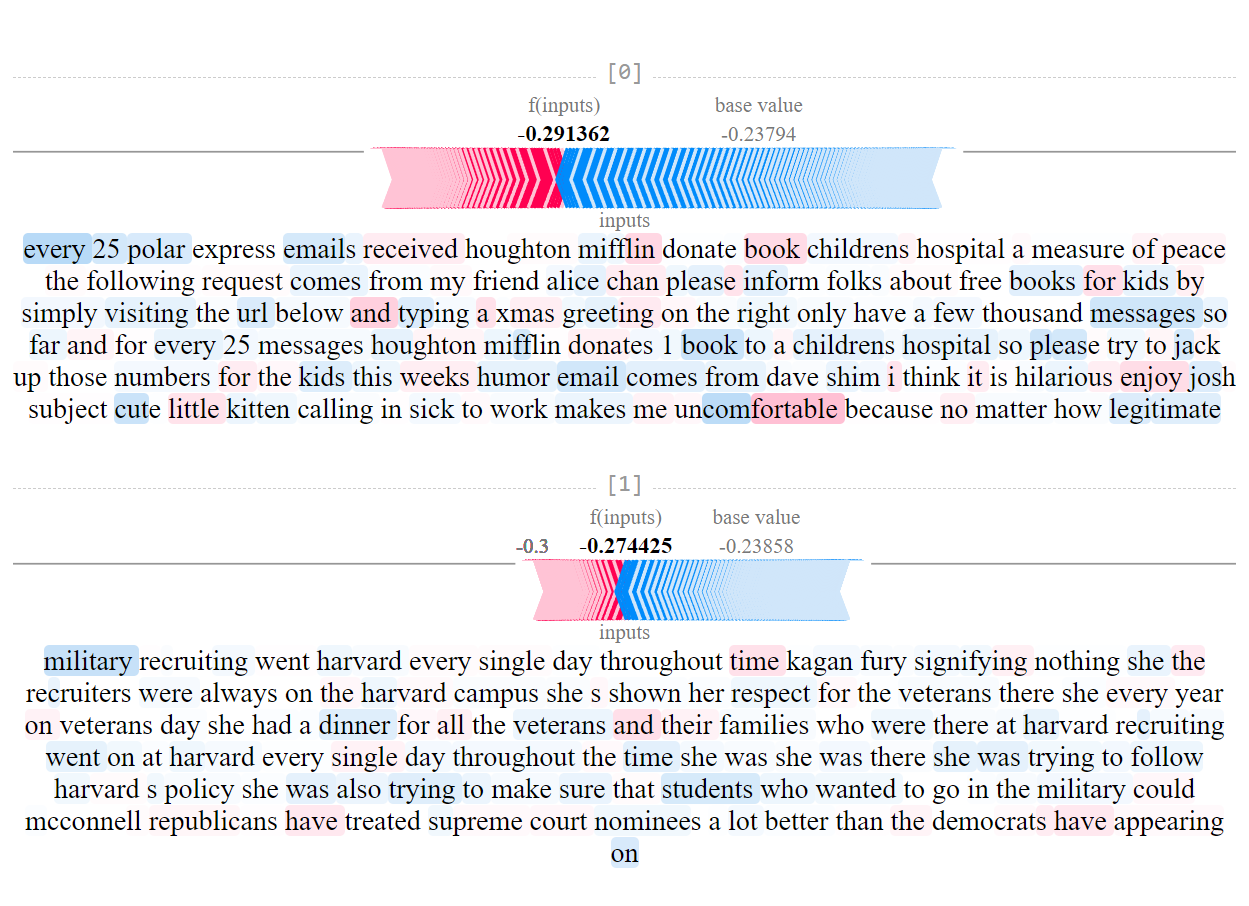
\includegraphics[width=\textwidth]{figs/one-distil-b-ml-c.png}
        % \caption{{DistilBERT}\textsubscript{B, C}}
    \endminipage\hfill % maximize horizontal separation
    \minipage{0.32\textwidth}
        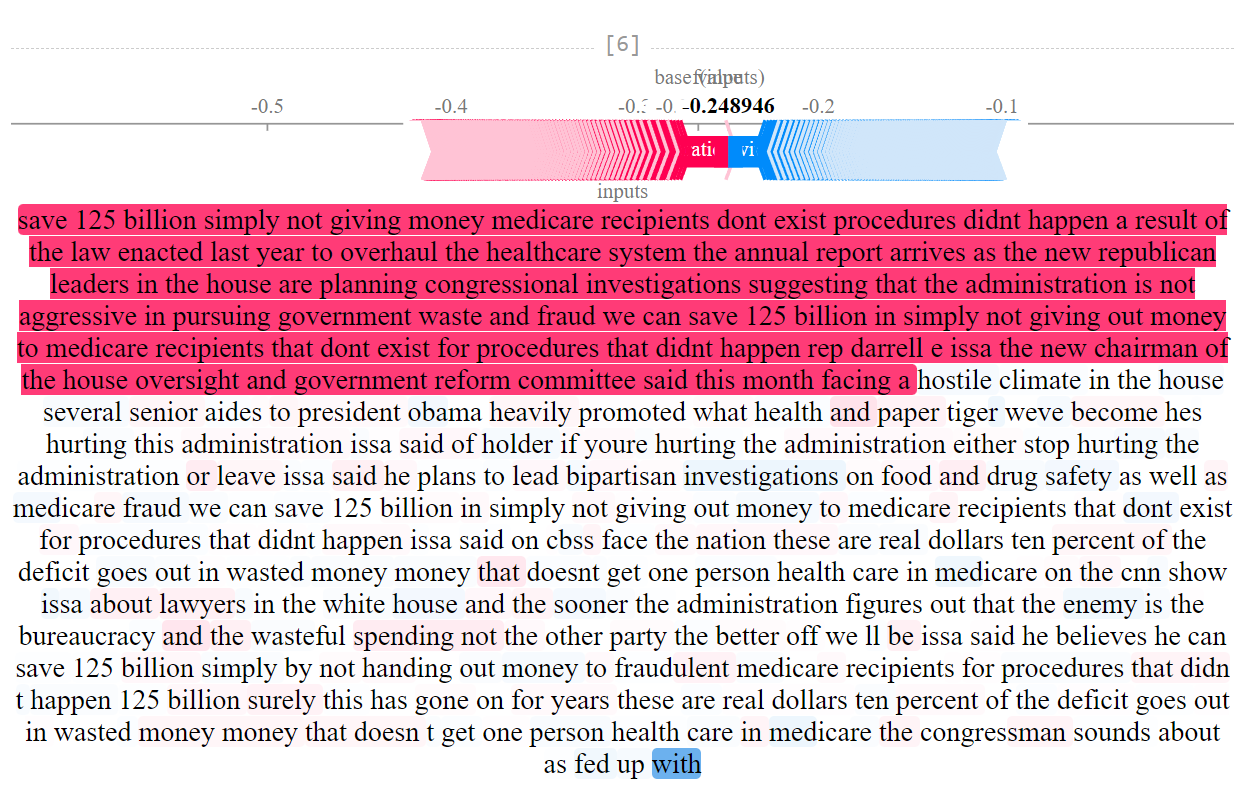
\includegraphics[width=\textwidth]{figs/all-distil-b-ml-c.png}
        % \caption{{DistilBERT}\textsubscript{B, C}}
    \endminipage\hfill % maximize horizontal separation
    \minipage{0.32\textwidth}
        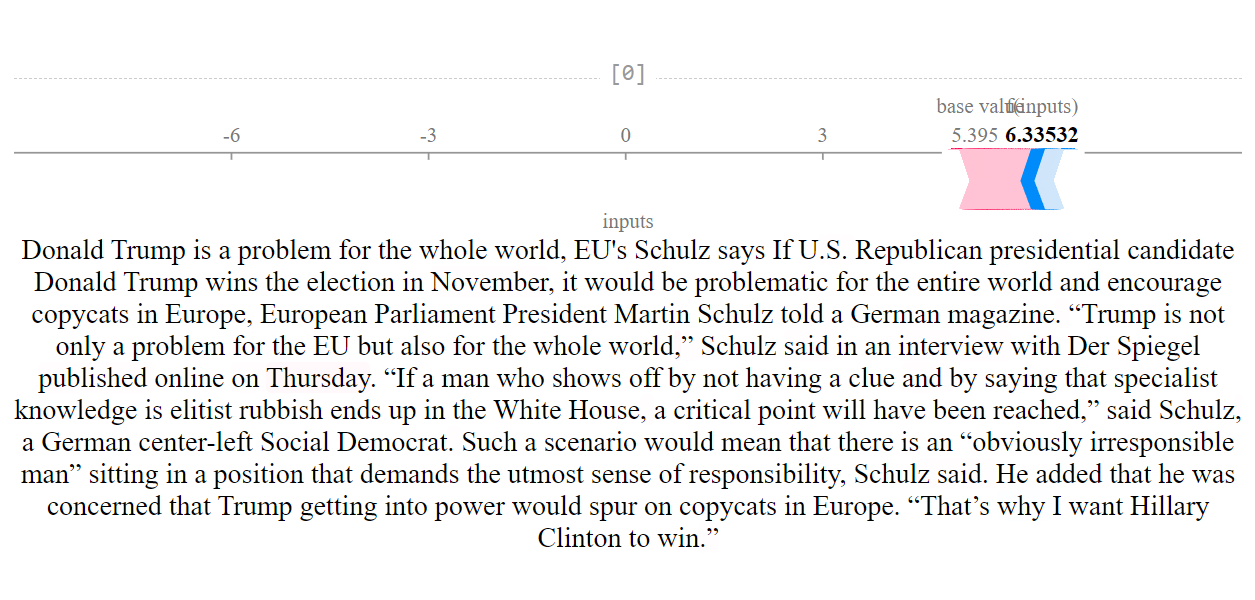
\includegraphics[width=\linewidth]{figs/news-distil-b-ml-c.png}
        % \caption{{DistilBERT}\textsubscript{B, C, ML}}
    \endminipage
    
    \caption{Valores Shapley de {DistilBERT}\textsubscript{B, C, ML} para los tres \textit{datasets}.}
    % \label{fig:shap-ps-one}
\end{figure}

\begin{itemize}
    \item LARGE, CASED, ML \textit{vs.} otros\footnote{Existen algunas excepciones según \textit{dataset} y modelo}.
    \item Rendimiento general: {P-S}\textsubscript{All} $>$ {P-S}\textsubscript{One} $>$ {News}.
\end{itemize}

\end{frame}

\begin{frame}{5.7. Evaluación}
\begin{itemize}
    \item LARGE ofrece resultados más consistentes.
    \item Alto valor de \textit{specificity}: gran capacidad de detectar noticias verdaderas.
    \item Análisis cuantitativo \textit{vs.} cualitativo: resultados generalmente poco concluyentes; distinto a lo esperado (\textit{datasets}, modelos...).
\end{itemize}
    
\end{frame}

\section{Discusión}
\section{Explicabilidad de los modelos}
\label{sec:expl}

El artículo de \citet{Dillon2021} recalca que hay que tener cuidado al interpretar los resultados obtenidos mediante técnicas como SHAP en búsqueda de conclusiones causales, ya que estas pueden ser erróneas o basarse en hechos infundados. Debido a que los modelos predictivos asumen ciertos comportamientos iguales en el futuro, los esquemas de correlación también se mantendrán constantes.

La revisión de \citet{Mosca2022} introduce otras técnicas basadas en valores Shapley, como \textit{L-Shapley} o \textit{C-Shapley}, y comenta críticas de otros trabajos hacia el uso en general del uso de valores Shapley en modelos de lenguaje que debatiremos a continuación.

\citet{Kumar2020} muestra que usar los valores Shapley puede provocar inconsistencias, las cuales añaden complexidad a los modelos que intentan mitigarlas. \citet{Merrick2019} critica la poca justificación o explicación en la incertidumbre en las explicaciones producidas mediante valores Shapley. En este caso muestran como pequeñas diferencias pueden generar efectos sobredimensionados en los resultados obtenidos, incluso en \textit{features} que no tienen relevancia en el modelo.

Cabe recalcar que estos trabajos no están directamente aplicados a tareas de Procesado de Lenguaje Natural. Aún así, consideramos necesario tener en cuenta estas perspectivas para contextualizar sobre todas los factores que influyen en el análisis de los resultados.

\section{Limitaciones de los modelos}

El trabajo de \citet{Rogers2020} ilustra los todos los conocimientos que se saben con respecto a los modelos basados en BERT en diferentes ámbitos.

\textbf{Conocimiento sintáctico.} BERT no `entiende'\ las negaciones y no es sensible al texto con una sintaxis incorrecta (orden de palabras aleatorizado, frases truncadas, sujetos o objetos eliminados \citep{Ettinger2019}

\textbf{Conocimiento semántico.} BERT tiene dificultades a la hora de trabajar con dígitos. Esto es problema del tokenizador WordPiece, que puede dividir números de valores similares de formas muy diferentes, afectando a todos los pasos posteriores del procesamiento y finalmente al resultado.

\textbf{Sentido común.} BERT no consigue llevar a cabo tareas de inferencia pragmática correctamente \citep{Ettinger2019} ni razonar a partir de su conocimiento del mundo \citep{Forbes2019, Zhou2019, Richardson2019}

Estos puntos mencionados dificultan el desarrollo de aplicaciones basadas en estas familias de modelos, concretamente el entrenamiento de modelos basado en hechos, ya que BERT tiene dificultades en el razonamiento. Aunque nuestra aplicación esté basada en características estilísticas, creemos que la falta de sensibilidad hacia las negaciones, estructuras sintácticas incorrectas o el problema a la hora de tratar con dígitos si que puede afectarnos en mayor o menor medida en los resultados obtenidos.


\section{Posibles sesgos}
\label{sec:biases}

En esta sección haremos una revisión bibliográfica sobre los trabajos realizados con respecto a determinar sesgos en LLMs.

\textbf{Word Embeddings estáticos y contextuales.} La investigación de \citet{Kurita2019} muestra que existen sesgos semánticos similares en \textit{word embeddings} contextuales al igual como sucede en los \textit{word embeddings} estáticos \citep{Caliskan2017}. Es más, el \textit{Word Embedding Associate Test} (WEAT) \citep{Caliskan2017}, no es directamente aplicable en estos modelos, debido a su naturaleza contextual. En el caso de aplicar esta métrica para reducir los sesgos en los modelos de lenguaje contextuales no es suficiente e incluso puede agravarlos aún más \citep{Silva2021}.

% \citet{Silva2021,Vig2020,Basta2019,Bommasani2020} han demostrado encontrar sesgos similares en este tipo de modelos basados en \textit{transformers}:

\textbf{Destilado de modelos.} Concretamente, los modelos destilados (en el caso de DistilBERT y DistilRoBERTa) muestran un sesgo estadísticamente mayor y más fuerte que en sus versiones no destiladas (BERT y RoBERTa) \citep{Silva2021}. Esto está en línea de los hallazgos de \citet{Hooker2020}, que encuentran que el proceso de destilado de modelos de visión daña desproporcionadamente a grupos minorizados. Aunque los trabajos de \citet{Gilburt2019,TanCelis2019} concluyen que aumentar el tamaño del modelo conlleva una reducción en el sesgo, \citet{Silva2021,Nadeem2021} demuestran lo contrario.

\textbf{Tokenización.} La tokenización es también crucial a la hora de desvelar sesgos: los modelos \textit{uncased}, es decir los que no distinguen entre palabras capitalizadas y no capitalizadas suelen mostrar menos sesgos y por lo tanto mayor diversidad con respecto a nombres y pronombres \citep{Silva2021}

\textbf{Modelos aumentados.} Mediante el trabajo de \citet{Vig2020}, podemos vislumbrar que los LLMs, concretamente las versiones aumentadas (véase las versiones LARGE de los modelos tratados a lo largo de este trabajo) tienen mayor capacidad de `sintetizar'\ o adquirir sesgos, aunque estos se manifiestan en una pequeña proporción de neuronas o \textit{attention heads}. El análisis cuantitativo desempeñado muestra que pueden existir componentes en estos modelos `encargados'\ explícitamente de reproducir sesgos o prejuicios (concretamente en este estudio solo se tratan estereotipos de género).

En conclusión, en este trabajo utilizamos modelos pre-entrenados basados en BERT, los cuales están demostrados que están sesgados. Es por ello que hay que tener en consideración para futuras investigaciones todos los factores que afectan al sesgo de los modelos para intentar reducirlo o en el caso de que no sea posible, tenerlo en cuenta en el análisis de los resultados.

\section{Conclusiones}
A continuación vamos a analizar cómo se han cumplido cada uno de los objetivos propuestos en la sección \hyperref[sec:objetivos]{1.2}:

\textbf{Definir correctamente el término \emph{fake news} y delimitar el área de estudio a tratar.} En el capítulo \hyperref[sec:defs]{2} hemos hecho una revisión bibliográfica, tomando diferentes definiciones del término y analizando los diferentes matices que aportan cada uno, decantándonos finalmente por el término de \textit{disinformation}, trabajando solamente noticias. Sabemos que nos dejamos muchas otras formas de \textit{disinformation}, pero es inevitable hacerlo debido a la naturaleza del Trabajo de Fin de Grado, es por ello que instamos a seguir investigando en el tema.

\textbf{Desarrollar una solución que permita clasificar noticias, sirviendo como triaje en el proceso de \textit{fact-checking}.} Se han propuesto diferentes modelos de lenguaje y \textit{datasets} y, viendo los resultados obtenidos en la sección \hyperref[sec:results]{6.1}, consideramos que hemos desarrollado un clasificador de noticias aunque los resultados no han sido los esperados. Los modelos LARGE, {DistilBERT}\textsubscript{B, C, ML}; {BERT}\textsubscript{B, C} y {DeBERTa}\textsubscript{B} son los que mejor funcionan en este problema, aunque creemos que los modelos implementados destacan más por sus métricas de \textit{specificity}, es decir, por su capacidad de distinguir qué características destacan en las noticias verdaderas. Aún así, por las métricas obtenidas en general, hace falta más trabajo para desarrollar una implementación que sea competente en el estado del arte actual.

\textbf{Hacer un estudio comparativo de los diferentes factores de los modelos y su aprendizaje, analizando la forma en la que afectan a su rendimiento.} En el capítulo \hyperref[chapter:6]{6} hemos comparado los diferentes resultados obtenidos y buscado una justificación plausible a este comportamiento. A grandes rasgos, el tamaño del modelo es el factor que parece contribuir más a la mejora de rendimiento de este. Lo segundo que parece afectar más es el hecho de si el modelo es multilingüe o distingue entre palabras capitalizadas. Por último, el tamaño del \textit{dataset} parece ser lo que menos contribuye, aunque hay que considerar la capacidad de generalización del modelo.

\textbf{Aplicar técnicas de \textit{Explainable AI} para entender el funcionamiento interno de los modelos en el proceso de clasificación.} En la sección \hyperref[sec:shap]{6.2} aplicamos estas técnicas mediante la librería \texttt{shap} y, mediante los valores Shapley, modelizamos la atención o la importancia que le da el modelo a ciertos \textit{tokens} en la clasificación. Concluimos que el comportamiento que tienen estos modelos no es el esperado, funcionando mejor en los \textit{datasets} {P-S}\textsubscript{One} y {P-S}\textsubscript{All} con menor información y número total de muestras que News. 
\newpage
\textbf{Analizar como afectan los sesgos en esta familia de modelos a los resultados obtenidos.} Como hemos observado en el apartado \hyperref[sec:biases]{7.2}, gracias a una revisión bibliográfica hemos conseguido desvelar sesgos en los LLMs. Estos no solo se limitan a una representación como \textit{word embedding} que puede dar interpretación a sesgos o prejuicios, sino que prácticamente estos sesgos son inherentes al proceso de aprendizaje. Es por ello que hay que tener en cuenta todos estos factores para realizar un análisis correcto de los resultados y de esta forma evitar perpetuando estos sesgos de forma directa e indirecta.

% \section{Trabajos futuros}
% % \begin{frame}{Trabajos futuros}
    
% \end{frame}

\section*{Bibliografía}
\begin{frame}[noframenumbering,plain,allowframebreaks]{Referencias}
        \printbibliography
\end{frame}

\end{document}

